\documentclass[11pt,a4paper]{report}
\usepackage[utf8]{inputenc}
\usepackage{amsmath}
\usepackage{amsfonts}
\usepackage{amssymb}
\usepackage{graphicx}
\usepackage[nottoc]{tocbibind}
\usepackage[semicolon]{natbib}
\usepackage{url}
\usepackage{listings}
\def\UrlBreaks{\do\/\do-}
\usepackage{breakurl}
\usepackage[breaklinks]{hyperref}
\bibliographystyle{unsrtnat}
\author{Aedan Lawrence \\\ \href{mailto:Aedan.Lawrence.2019@live.rhul.ac.uk}{Aedan.Lawrence.2019@live.rhul.ac.uk}}
\title{Combating Fake News Using Mobile Trusted Execution Environments}
\date{EPMS School, Royal Holloway University of London, Egham TW20 0PW, UK}
\begin{document}
\maketitle
\tableofcontents
\newpage
\section{Abstract}
\textbf{On messaging apps such as WhatsApp news can get shared into large groups which people can and do take a face value without critically thinking.} If a malicious figure were to pretend to be a trusted news agency this can allow for the fake news to spread very quickly. Therefore, we need a way to detect fake news which is trying to masquerade as a trusted news source.

Fake news has gained a large amount of publicity over the recent years, however current detection methods use langue analysis and some common sense. This however can mean that people can often fail to detect fake news correctly.

My approach to fixing this is to design and prototype a system that allows me to receive a link, check that link compared to a list of the news source, verify that the news source indeed wrote that article and therefore sign the article using a private key which would allow the messaging group to know that this comes from a valid news source taking out some of the guessing work in spotting fake news. This checking could also be offloaded to the phones TEE chip which would allow for it to be even more secure.

Finally, this solution is a tiny step in trying to stop the spread of fake news and is not a solution on its own. However, mixed with other pre-existing technologies to detect fake news it is a steppingstone in trying to limit its effects. 

\newpage
\section{Introduction}
Fake news has been an issue for many years, it is getting increasingly prevalent in everyday life and therefore detection methods need to get better as well as more accurate. A report by First Draft News \citep{Fakenews} identified seven distinct types of fake news these are:
\begin{enumerate}
  \item satire or parody.
  \item false connection.
  \item misleading content.
  \item false context.
  \item imposter content.
  \item manipulated content.
  \item fabricated content.
\end{enumerate}
Typically, most news will be shared via social media and messaging applications, this can give people in charge of groups on these sites a large amount of power over what news people see, share, and read. As of 2021 13\% of all news that is read will be from Facebook alone \citep{Echobox}. With the rise in influence social media has over our lives whether that be political such as the 2016 US election or medical-related such as, during the COVID-19 pandemic, we need to manage and correctly identify information that is being shared. Facebook started this during the pandemic, flagging miss-leading news as potentially inaccurate on all social media platforms that it owned.

I plan on being able to help identify news sources that are satire or parody in nature as well as impostor content as both will be detectable based upon the URL and certificates. This would be implementable into most social media and messaging apps and allow for articles to be flagged as potentially imposter or known satire content. This is especially useful as want to be imposters can easily make their domain look something like bbc.a.co.uk which for the typical person may be hard to spot anything that would suggest that is not the BBC.

The project started by planning a system to implement which looks something like this:
\begin{center}
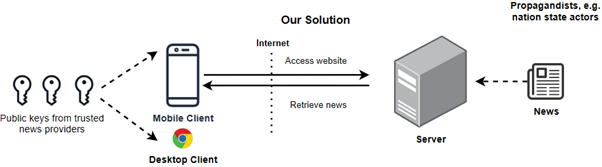
\includegraphics[width=1\textwidth]{image/diagram.png}
\end{center}

The plan here is when a URL is shared of an expected to be news website then the phone will send a request to the server.

As I will only be prototyping this system due to time constants, I picked Flask for python as my framework for the server. This allows for rapid changes and easy development. As well as Flask I will be using the cryptography module for python as this allows me to easily sign the news content using ECDSA (Elliptic Curve Digital Signature Algorithm). Finally, I will also make use of SQLAlchemy to store the keys which each publisher can use.

Why ECDSA? ECDSA while being less commonly used overall is more complicated due to its asymmetry this means it is harder to revert. “ECDSA provides the same level of security as RSA, but it does so while using much shorter key lengths. Therefore, for longer keys, ECDSA will take considerably more time to crack through brute-forcing attacks.” \citep{RSA}. It can however be harder overall to implement which may cause issues in development.

Once this is working my next task will be to modify an Android application to make use of this signing server when it detects a news article being shared on the platform. An easy proof of concept way to do this will be to detect and check all URL’s that are being shared on the platform. This way all news content will be flagged, and non-news links will be marked with a warning.

Once a URL is detected, a query to the signing server needs to be made providing the URL which has been shared via social media. This allows the signing server to try and match that URL with known good news sources, if it can then find that article on a news site, we know that it is a real article and not an imposter article.

Once found the signing server will sign the URL and return that information to the requesting application. It is then up to the application to check the signature using the server’s public key and at that point can confirm to the user that this is indeed news from the claimed publisher.

Parody news sites can be checked in the same way, but the returning information will just have an additional flag to mark it as parody content. This then allows the end-user application to flag it as a known parody site.

To allow for this to be even more secure the handling of decoding the signature could be done using the phones TEE chip which would make this system much harder to penetrate. This could be modelled on Linux using OP-TEE (Open Portable Trusted Execution Environment).

According to OP-TEE’s documentation, it helps to separate the non-secure OS and user apps from the secure code which is baked into the hardware \citep{OP-TEE}. This would allow the singing verification code to run securely without the worry of being tampered with. This will help to have an even higher level of validity for the news checking.

Once I have finished the working prototype of the signing server and Android application, I will look at prototyping an OP-TEE application which decodes the signature so that in a perfect world the three could be combined making a functional verification service with the security of TEE (Trusted Execution Environment).
\newpage
\section{Development and Difficulties}
\subsection{Flask Server}
The python server implementation was smooth and required little coding expertise in this basic proof of concept method.

A key issue which showed its head early on was the lack of free and publicly accessible APIs (Application Programming Interfaces) from publishers, this limited the project in the number of working sites in the prototype. Due to not having the time to email each publisher separately I used two API’s I could get by just signing up for publicly, this was the New York Times and The Guardian. In a perfect world I would have had access to all news publishers instead of just these two.

This was also an issue for spotting a satirical/parody news website as it meant I could only spot them using string matching on the domain name and therefore could not check whether it was just a parody news site or an imposter site pretending to be a parody news website. This however is not the end of the world as it still detects most parody websites and worst case they will be flagged as possibly imposter/uncheckable instead of parody.

In the end, I fixed both issues by writing my own API for news websites. By storing the certificates of a trusted news source, I can compare the incoming URL with my certificate store and if there is a match and the URL returns a 200-response code then I can sign the news. This allows me to check websites which do not provided an API.

Now I can simply add public keys of trusted news sources to my database, and I can start verifying all news sources.

A working a json reply can look like:
\begin{center}
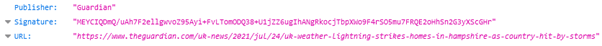
\includegraphics[width=1\textwidth]{image/json1.png}
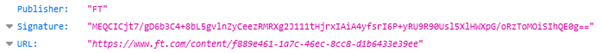
\includegraphics[width=1\textwidth]{image/json2.png}
\end{center}

Another issue I faced was sharing the public key so that the mobile client could easily access it. This is due to Flask only allowing for returns to be a string, dict, tuple, Response instance or WSGI callable. With a bit of research, I found I could share the public key in bytes form using the public\_bytes() method built into the EC (Elliptic Curve) Cryptography package. Typically, this would not be an issue as the public key would be collected from a trusted certificate store and therefore would not need to be shared by the server.

However, after playing with this for a while, I realised I was wasting my time and should have been hard coding the public key to verify the signature as it does not need to change or expire for testing purposes and therefore can just be stored within the java application.
\newpage
\subsection{Signal Application}
My next challenge was to pick an application to modify to implement this system. The obvious choice would have been messenger and WhatsApp however both apps are closed source and therefore I had to look elsewhere. This led me to finding signal \citep{Signal} has exceptionally good open-source support. As it is effectively a mirror application of WhatsApp however not being owned by Facebook it was a suitable candidate to show an example implementation.

First, I had to isolate the URL handling part of Signal, filtering through methods in android studio this led me to find linkpreview in the securesms package. The methods in the LinkPreviewUtil class are called every time a preview for a URL needs to be loaded. By modifying this class, I can get access to just the URL part of the message which has been sent.

Next while in a development stage I disabled the requirement for the HTTPS certificate to be stored with a certificate store as this is a requirement for Android apps however would have just cost me money to test this idea, having not done much android app development before I also disabled the requirement for URL responses to be done using background threads as it was simpler just to wait for a response. Once I had a working verification method, I put the requests to my server in an AsyncTask which allowed me to reenable Android’s thread requirements. 

This allows me to send the two needed requests to the server, first to provide the URL and then to get the public key to check the signature of the response. The next step is to take the provided information from the server and using java’s built-in security packages recreate the public key and then verify the provided signature.

While reconstructing the public key and signature in java I was having a tough time getting a working, parseable public key. After doing some research this is due to the way hazmat cryptography handles EC encryption by default vs how Java Security handles EC encryption.

While python has very good support for different types of curves java on Android does not. This meant I was providing java with a secp256k1 curve which java could create a public key from however could not use to verify the signature. One of the few curve’s java supports is secp256r1 so once I converted my server key to this format java could easily verify the signature. \citep{Exception}.

Finally, this meant I could verify news sources sent via Signal on android, if an URL is pretending to be a news source that it is not then it will not be verified. At this moment in time, it only is verifiable using the ADB logs and does not have a visual display element. To get a visual display I need to add a Snackbar to the application, this will allow for a little pop up to alert the user if the news source is valid or not.
\newpage
\subsection{Current Known Bugs and Limitations}
\begin{enumerate}
  \item Not all news websites can be added to my own API as the way I read the public certificate does not work with all certificates for some reason.
  \item The URL is checked every time the preview for a URL is loaded, this means if the news site goes down after it has been sent and received once, it could later be flagged as possible imposter news.
  \item The NYTimes is using their API, this limits me to being able to check the top 20 articles of the day. The Guardian’s API on the other hand just seems to fail for some articles with no apparent reason.
  \item All network request that goes through signal will accept their certificates even if they are self-signed currently due to the implementation of talking to my server. This is not secure!
  \item Due to time constraints all code is not heavily debugged and can error on edge cases when it shouldn’t.
\end{enumerate}
\newpage
\section{Conclusion and Reflection}
\textbf{Overall, I think this project in its current state has gone quite well. The fundamental problem of having to manually spot impostor news has been accomplished.} Also adding the ability to spot satire news helps to stop the spread of miss information even if unintentionally.

However, as of the time writing this report, I have not yet had the opportunity to look at or start to implement OP-TEE. This means there is still a bit of work to be made in making the system more secure. If I was to start this project again, I would work on this implementation before the Android one as the two are linked. This could be start by running getting OP-TEE running on QEMU to emulate an arm device.

Another main implementation of this system would be to get it added to bigger/other social media applications as well as desktop add on for web browsers. This would allow news link on any website to be checked for being imposter/satire news, while not helpful for all users this may be helpful for older generations, as a web browser.

I also spent to long research and not asking enough questions, this wasted my own time as I would be trying to implement ideas that were not need and/or not helpful. As this was such a practical based UROP (Undergraduate Research Opportunities) if I was to do it again, I would jump straight into development and do research at the same time instead of a few weeks of research followed by a few weeks of coding. I would also have a higher interaction with my lectures which would help to mitigate these issues.

Yet another thing which could be done would be to combine this detection system with a language analysis method of detecting fake news. As this would allow many more websites to be flagged for things which are not just imposter content.

I am however happy with the technologies I have learned to use along the way such as elliptical curve encryption, Flask servers and android app development. As these are all things which before the project, I had ether not done or done to a much lower level.
\newpage
\section{Code availability}
The python server code can be found here: \\ \url{https://github.com/MrInterBugs/Combatting-Fake-News} \\ The modified signal code can be found here: \\ \url{https://github.com/MrInterBugs/Signal-Android}
\newpage
\bibliography{References}
\end{document}